\documentclass[border=3mm]{standalone}
\usepackage{tikz}
\usetikzlibrary{arrows, shapes.gates.logic.US, shapes.gates.logic.IEC, calc}

\tikzset{
    my-nand-gate/.style={
        nand gate US, draw, rotate=0, logic gate inputs=nn
    },
    my-branch/.style={
        fill, shape=circle, minimum size=3pt, inner sep=0pt
    },
}

\begin{document}

\resizebox{16cm}{!}{

    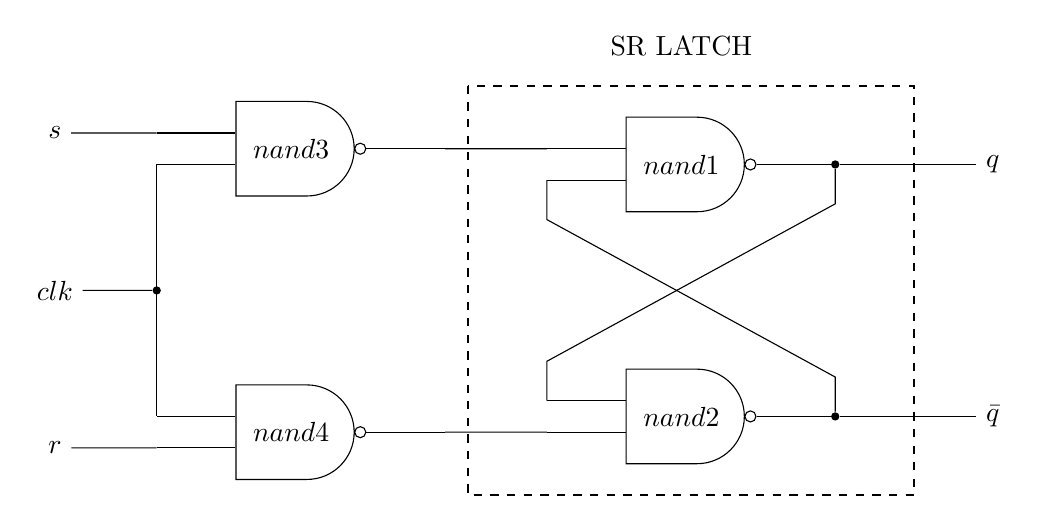
\begin{tikzpicture}[label distance=2mm]

        % INPUTS
        \node[] (S)   at (0,4) {\normalsize $s$};
        \node[] (CLK) at (0,2) {\normalsize $clk$};
        \node[] (R)   at (0,0) {\normalsize $r$};

        % NAND3, WIRES AND CONNECTOR POINTS
        \node[my-nand-gate] (NAND3)    at ($(S) + (3, -.2)$)            {\normalsize $nand3$};
        \coordinate[]       (NAND3IN1) at ($(NAND3.input 1) + (-1, 0)$) {};
        \coordinate[]       (NAND3IN2) at ($(NAND3.input 2) + (-1, 0)$) {};
        \coordinate[]       (NAND3OUT) at ($(NAND3.output)  + (1, 0)$)  {};
        \draw (NAND3.input 1) -- (NAND3IN1);
        \draw (NAND3.input 2) -- (NAND3IN2);
        \draw (NAND3.output)  -- (NAND3OUT);
        
        % NAND4, WIRES AND CONNECTOR POINTS
        \node[my-nand-gate] (NAND4)    at ($(R) + (3, .2)$)             {\normalsize $nand4$};
        \coordinate[]       (NAND4IN1) at ($(NAND4.input 1) + (-1, 0)$) {};
        \coordinate[]       (NAND4IN2) at ($(NAND4.input 2) + (-1, 0)$) {};
        \coordinate[]       (NAND4OUT) at ($(NAND4.output)  + (1, 0)$)  {};
        \draw (NAND4.input 1) -- (NAND4IN1);
        \draw (NAND4.input 2) -- (NAND4IN2);
        \draw (NAND4.output)  -- (NAND4OUT);

        % NAND1, WIRES AND CONNECTOR POINTS
        \node[my-nand-gate] (NAND1)    at ($(NAND3OUT) + (3, -.2)$)            {\normalsize $nand1$};
        \coordinate[]       (NAND1IN1) at ($(NAND1.input 1) + (-1, 0)$) {};
        \coordinate[]       (NAND1IN2) at ($(NAND1.input 2) + (-1, 0)$) {};
        \node[my-branch]    (NAND1OUT) at ($(NAND1.output)  + (1, 0)$)  {};
        \draw (NAND1.input 1) -- (NAND1IN1);
        \draw (NAND1.input 2) -- (NAND1IN2);
        \draw (NAND1.output)  -- (NAND1OUT);
        
        % NAND2, WIRES AND CONNECTOR POINTS
        \node[my-nand-gate] (NAND2)    at ($(NAND4OUT) + (3, .2)$)             {\normalsize $nand2$};
        \coordinate[]       (NAND2IN1) at ($(NAND2.input 1) + (-1, 0)$) {};
        \coordinate[]       (NAND2IN2) at ($(NAND2.input 2) + (-1, 0)$) {};
        \node[my-branch]    (NAND2OUT) at ($(NAND2.output)  + (1, 0)$)  {};
        \draw (NAND2.input 1) -- (NAND2IN1);
        \draw (NAND2.input 2) -- (NAND2IN2);
        \draw (NAND2.output)  -- (NAND2OUT);

        % OUTPUTS
        \node[] (Q)    at ($(NAND1OUT) + (2, 0)$) {\normalsize $q$};
        \node[] (QBAR) at ($(NAND2OUT) + (2, 0)$) {\normalsize $\bar{q}$};
                
        % INPUT CONNECTIONS
        \draw (S) -- (NAND3IN1);
        \draw (R) -- (NAND4IN2);
        
        % OUTPUT CONNECTIONS
        \draw (NAND1OUT) -- (Q);
        \draw (NAND2OUT) -- (QBAR);

        % INTERNAL WIRES - NAND GATES
        \draw (NAND3OUT) -- (NAND1IN1);
        \draw (NAND4OUT) -- (NAND2IN2);
        \draw (NAND1OUT) -- ++(0,-0.5) -- ($(NAND2IN1) +(0,0.5)$)  -- (NAND2IN1);
        \draw (NAND2OUT) -- ++(0,0.5)  -- ($(NAND1IN2) +(0,-0.5)$) -- (NAND1IN2);

        % INTERNAL WIRES - CLOCK
        \draw (NAND3IN2) -- (NAND4IN1) node[my-branch, pos=1/2] (CLKBRANCH) {};
        \draw (CLK) -- (CLKBRANCH);

        % DRAW DOTTED LINE BOX AROUND SR LATCH
        \draw[thick, dashed] ($(NAND1IN1) + (-1, .8)$) rectangle ($(NAND2OUT) + (1, -1)$);
        \node[] at ($(NAND1) + (0, 1.5)$) {\normalsize SR LATCH};

    \end{tikzpicture}
}

\end{document} 
